\documentclass[conference]{IEEEtran}

% ---------------------------------------------------------------------------
% Standard IEEE packages
% ---------------------------------------------------------------------------
\usepackage{amsmath,amssymb}
\usepackage{graphicx}
\usepackage{booktabs}
\usepackage{cite}
\usepackage{microtype}
\usepackage{algorithm}
\usepackage{algpseudocode}
\usepackage{xcolor}
\usepackage{hyperref}
\usepackage{balance}
\hypersetup{colorlinks=true,linkcolor=blue,citecolor=blue,urlcolor=blue}

% ---------------------------------------------------------------------------
% Notation helpers
% ---------------------------------------------------------------------------
\newcommand{\Tsparse}{T_{\mathrm{sparse}}}
\newcommand{\Tdense}{T_{\mathrm{dense}}}
\newcommand{\Tfusion}{T_{\mathrm{fusion}}}
\newcommand{\Thydrate}{T_{\mathrm{hydrate}}}
\newcommand{\Tprefill}{T_{\mathrm{prefill}}}
\newcommand{\Twan}{T_{\mathrm{WAN}}}
\newcommand{\Tttft}{T_{\mathrm{TTFT}}}
\newcommand{\Tdecode}{T_{\mathrm{decode}}}
\newcommand{\Rdecode}{R_{\mathrm{decode}}}
\newcommand{\pwan}{p}

\begin{document}

\title{Geo-Distributed Hybrid Retrieval-Augmented Generation:\\
Placement Tradeoffs and Speculative Prefill Acceleration}

\author{\IEEEauthorblockN{M.~Abdullah Ali\IEEEauthorrefmark{1},
M.~Abdullah Aamir\IEEEauthorrefmark{1}}
\IEEEauthorblockA{\IEEEauthorrefmark{1}Department of Data Science,
FAST-NUCES, Islamabad, Pakistan\\
\{m.abdullah.ali, m.abdullah.aamir\}@fast.edu.pk}}

\maketitle

% ===========================================================================
%  ABSTRACT
% ===========================================================================
\begin{abstract}
Retrieval-Augmented Generation (RAG) systems are increasingly deployed across
geographically distributed, heterogeneous nodes, yet the placement of their
individual pipeline stages---sparse retrieval, dense retrieval, fusion,
hydration, and generation---remains an open systems question. We present the
first factorial measurement study of stage-to-node placement for a \emph{hybrid}
RAG pipeline (BM25 + BGE-M3 dense retrieval with reciprocal-rank fusion) on
commodity hardware: an RTX~3090 generation host and a GTX~1660~Ti laptop
gateway, connected over a WireGuard link and shaped with Linux \texttt{netem}
across four WAN regimes (0/15/40/80~ms). Our characterization exposes a striking
\emph{asymmetric leg disparity}: the sparse leg completes in $\approx$120~ms
while the dense leg takes $\approx$2256~ms, a 19$\times$ gap that dominates
time-to-first-token (TTFT) and makes naive parallelism ineffective. We exploit
this asymmetry with \textbf{SPHP} (Speculative Progressive Hydration \&
Prefill), a protocol that transmits a provisional sparse hint to the generation
node, runs a masked speculative prefill that overlaps the slow dense leg, and
reconciles against the fused context on arrival, reducing TTFT by 6.2--6.5\%
with no change in retrieval quality. We further derive an analytical placement
cost model for four topologies (P0--P3) whose component-level predictions match
held-out measurements to 4.18\% MAPE, and use it to produce a crossover map
showing that the SPHP-augmented split placement is optimal across the entire
swept (RTT, bandwidth) space. All artifacts are released for reproducibility.
\end{abstract}

\begin{IEEEkeywords}
Retrieval-Augmented Generation; hybrid search; edge--cloud systems;
speculative decoding; geo-distributed inference; placement optimization.
\end{IEEEkeywords}

% ===========================================================================
%  I. INTRODUCTION
% ===========================================================================
\section{Introduction}
\label{sec:intro}

Retrieval-Augmented Generation (RAG) has become the dominant architecture for
grounding large language models (LLMs) in external knowledge
\cite{lewis2020rag,guu2020realm,borgeaud2022retro,gao2024ragsurvey}. A modern
RAG pipeline is not a single monolith but a sequence of heterogeneous stages:
a \emph{sparse} lexical search (e.g., BM25 \cite{robertson1994bm25}), a
\emph{dense} semantic search over learned embeddings
\cite{karpukhin2020dpr,reimers2019sbert,chen2024bge}, a \emph{fusion} step that
merges the two ranked lists (e.g., reciprocal-rank fusion
\cite{cormack2009rrf}), a \emph{hydration} step that fetches the full text of
the selected passages, and finally \emph{generation}, in which an LLM
\cite{vaswani2017transformer,brown2020gpt3,llama2024} is prefilled with the
retrieved context and autoregressively decodes an answer
\cite{kwon2023vllm,lin2024awq}.

As these systems move from a single datacenter box to the edge, a fundamental
\emph{placement dilemma} emerges. The stages have wildly different resource
profiles: dense retrieval and generation demand a GPU, sparse retrieval is
CPU-friendly, and hydration is a cheap disk lookup. Large models require
hardware most machines do not have, data-residency rules can force retrieval
and generation onto different hosts, and cost pushes work toward whatever
hardware exists. Yet, to the best of our knowledge, the literature cannot
answer: \emph{where should each stage of a hybrid RAG pipeline run, under which
network conditions, and what exactly is lost when the topology degrades?}
DNN partitioning is studied at the layer level
\cite{kang2017neurosurgeon,hung2020cloudedge,zhang2021cloudedge} and LLM
serving splits model \emph{phases} across machines, but a measurement study of
\emph{which pipeline stage runs on which machine} in a multi-node hybrid RAG
deployment is missing.

We close this gap with a deployed, instrumented two-node testbed and a
factorial campaign over placement $\times$ network regime. Our contributions
are:

\begin{itemize}
\item \textbf{C1 (Measurement).} The first factorial measurement of
stage-to-node placement for hybrid RAG on commodity heterogeneous hardware
(RTX~3090 + GTX~1660~Ti) over a WireGuard link shaped by \texttt{netem}
\cite{donenfeld2017wireguard,hemminger2000netem} across four WAN regimes. We
quantify the \emph{asymmetric leg disparity}---a 120~ms sparse leg versus a
2256~ms dense leg---that governs TTFT and renders naive parallel overlap
ineffective (\S\ref{sec:characterization}).

\item \textbf{C2 (Mechanism).} \textbf{SPHP}, a speculative protocol that
converts the leg disparity from a liability into an opportunity: a provisional
sparse hint is shipped to the generation node, a masked speculative prefill
runs in parallel with the slow dense leg, and the result is reconciled against
the fused context on arrival. SPHP reduces TTFT by 6.2--6.5\% at zero retrieval
quality cost (\S\ref{sec:sphp}).

\item \textbf{C3 (Model).} An analytical placement cost model for four
topologies (P0--P3) whose component-level predictions match held-out
measurements to 4.18\% MAPE, together with a crossover map showing the
SPHP-augmented split placement is optimal across the entire swept (RTT,
bandwidth) space (\S\ref{sec:costmodel}).

\item \textbf{C4 (Artifacts).} A fully open, reproducible testbed: the
8.84M-passage MS~MARCO index \cite{bajaj2018msmarco}, the benchmark harness,
the cost model, and all figures (\S\ref{sec:discussion}).
\end{itemize}

The remainder of the paper is organized as follows.
\S\ref{sec:related} reviews related work on RAG, hybrid retrieval,
speculative inference, and edge--cloud systems. \S\ref{sec:architecture}
describes the two-node deployment and the placement taxonomy.
\S\ref{sec:characterization} presents the empirical characterization,
including the asymmetric leg disparity. \S\ref{sec:sphp} details the SPHP
protocol. \S\ref{sec:costmodel} develops the analytical placement cost model
and the crossover map. \S\ref{sec:evaluation} reports the evaluation, and
\S\ref{sec:discussion}--\S\ref{sec:conclusion} discuss the results and
conclude.

% ===========================================================================
%  II. RELATED WORK
% ===========================================================================
\section{Related Work}
\label{sec:related}

\subsection{Retrieval-Augmented Generation}
RAG couples a parametric generator with a non-parametric memory. Lewis
\emph{et al.}~\cite{lewis2020rag} introduced the generator--retriever
formulation for knowledge-intensive tasks; REALM~\cite{guu2020realm} and
RETRO~\cite{borgeaud2022retro} showed that retrieving from trillions of tokens
improves language modeling at scale. A recent survey
\cite{gao2024ragsurvey} organizes the field into naive, advanced, and
modular RAG, and active-retrieval variants such as FLARE
\cite{jiang2023flare} and the declarative compiler DSPy \cite{khattab2023dspy}
adapt retrieval to the query. All of this work assumes a single, well-provisioned
host; none addresses the placement of the retrieval and generation stages
across a geo-distributed, heterogeneous fleet.

\subsection{Hybrid Retrieval and Fusion}
Hybrid search combines a lexical (sparse) and a semantic (dense) signal. BM25
\cite{robertson1994bm25} remains the lexical workhorse; dense passage retrieval
\cite{karpukhin2020dpr} and sentence embeddings \cite{reimers2019sbert} provide
the semantic leg, with multi-vector late-interaction models such as ColBERT
\cite{khattab2020colbert} improving effectiveness at higher cost. Modern
multi-functionality embedding models such as BGE-M3 \cite{chen2024bge} serve
both dense and lexical objectives from one encoder. Reciprocal-rank fusion
\cite{cormack2009rrf} is the standard parameter-light combiner. We use exactly
this stack---Tantivy BM25, BGE-M3 dense search over Qdrant, and RRF---and
measure how its two legs behave when split across machines.

\subsection{Speculative LLM Inference}
Speculative decoding accelerates autoregressive generation by drafting with a
cheap model and verifying with a large one
\cite{leviathan2023speculative,chen2023speculative}. Our SPHP mechanism is
\emph{orthogonal} to this line: rather than speculating over the
\emph{tokens} of a single model, we speculate over the \emph{pipeline
schedule}---we begin prefilling the generation node on a provisional (sparse)
context before the expensive dense leg has finished, then mask and reconcile.
This is a form of pipeline-level speculation that exploits the leg disparity
measured in \S\ref{sec:characterization}.

\subsection{Edge--Cloud and Geo-Distributed Systems}
Hybrid cloud--edge inference partitions a network between a device and a
server \cite{kang2017neurosurgeon,hung2020cloudedge,zhang2021cloudedge}, and
datacenter-scale serving systems study phase and memory management
\cite{kwon2023vllm,zaharia2016datacenter}. Secure point-to-point tunnels such
as WireGuard \cite{donenfeld2017wireguard} and kernel traffic control
(\texttt{tc}/\texttt{netem}) \cite{hemminger2000netem} provide the transport
and the controlled-WAN substrate we use. Energy and policy considerations for
distributed deep learning \cite{strubell2019energy} motivate placing expensive
stages where hardware and power are cheapest. Our work is the first to bring
this placement lens to the RAG pipeline itself.

% ===========================================================================
%  III. SYSTEM ARCHITECTURE & DEPLOYMENT
% ===========================================================================
\section{System Architecture \& Deployment}
\label{sec:architecture}

\subsection{Testbed}
We deploy a two-node hybrid RAG system over a WireGuard virtual private
network. \textbf{Node~A} (generation) is an RTX~3090 workstation
(24~GB VRAM) running a LLaMA-3-8B-Instruct model quantized with AWQ
\cite{lin2024awq,llama2024} under vLLM \cite{kwon2023vllm}, together with a
local SQLite store holding the full 8{,}841{,}823-passage MS~MARCO corpus
\cite{bajaj2018msmarco} for $O(1)$ hydration. \textbf{Node~B} (edge gateway)
is a laptop (Intel i7-10750H, GTX~1660~Ti) running the retrieval stack: a
Tantivy BM25 index over the full 8.84M passages, a BGE-M3 dense encoder
\cite{chen2024bge} with a 1024-dimensional HNSW index in Qdrant, and local
reciprocal-rank fusion \cite{cormack2009rrf}. The two nodes are connected over
WireGuard \cite{donenfeld2017wireguard} (Node~A at 10.8.0.1, Node~B at
10.8.0.5) with gRPC streaming for the query, the fused context, and the
returned token stream. Figure~\ref{fig:arch} shows the architecture and the
per-stage timing annotations.

\begin{figure*}[t]
\centering
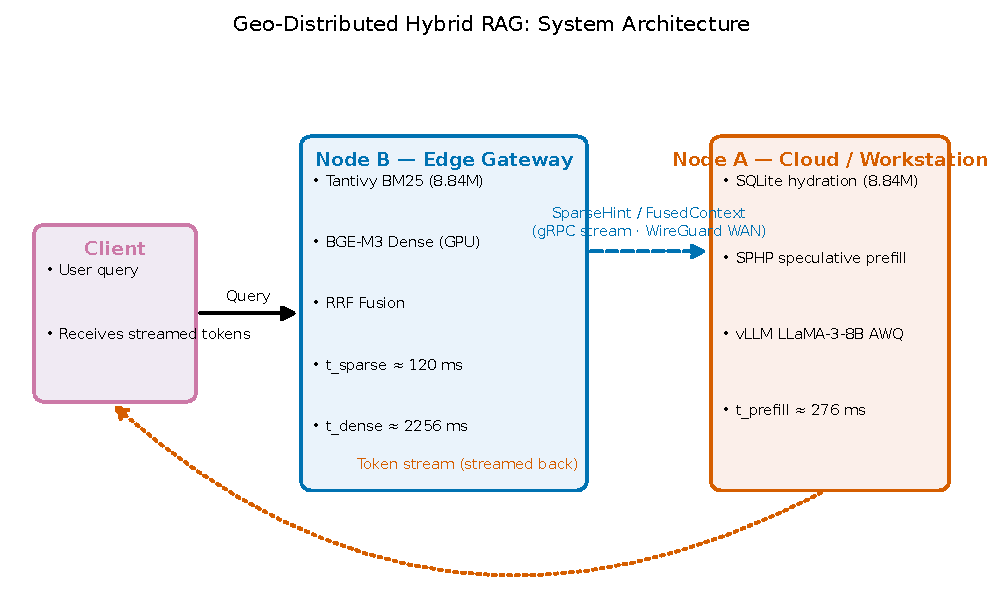
\includegraphics[width=\textwidth]{figures/fig1_arch.pdf}
\caption{System architecture. The client query enters the edge gateway
(Node~B), which runs sparse (Tantivy BM25) and dense (BGE-M3/Qdrant) retrieval
in parallel and fuses them with RRF. The fused context (or a provisional
sparse hint under SPHP) is streamed over the WireGuard WAN to the generation
host (Node~A), which hydrates the passages from local SQLite and runs the
AWQ-quantized LLaMA-3-8B under vLLM. Tokens are streamed back to the client.}
\label{fig:arch}
\end{figure*}

\subsection{Placement Topologies}
We define a taxonomy of five placement topologies by the location of the
pipeline boundary (Figure~\ref{fig:topologies}):
\textbf{P0} (colocated) runs every stage on Node~A; \textbf{P1} places only the
gateway on Node~B with all compute on Node~A; \textbf{P2} (our baseline) runs
sparse, dense, and fusion on Node~B and hydration, prefill, and decode on
Node~A, shipping only the top-$k$ document identifiers across the WAN;
\textbf{P2-SPHP} augments P2 with the speculative protocol of
\S\ref{sec:sphp}; and \textbf{P3} moves hydration to Node~B as well, shipping
the full text of the top passages. P2 is the natural split: it keeps the
GPU-bound dense retrieval and generation on capable hardware while moving the
cheap identifier payload---not the bulky corpus text---across the link.

\begin{figure*}[t]
\centering
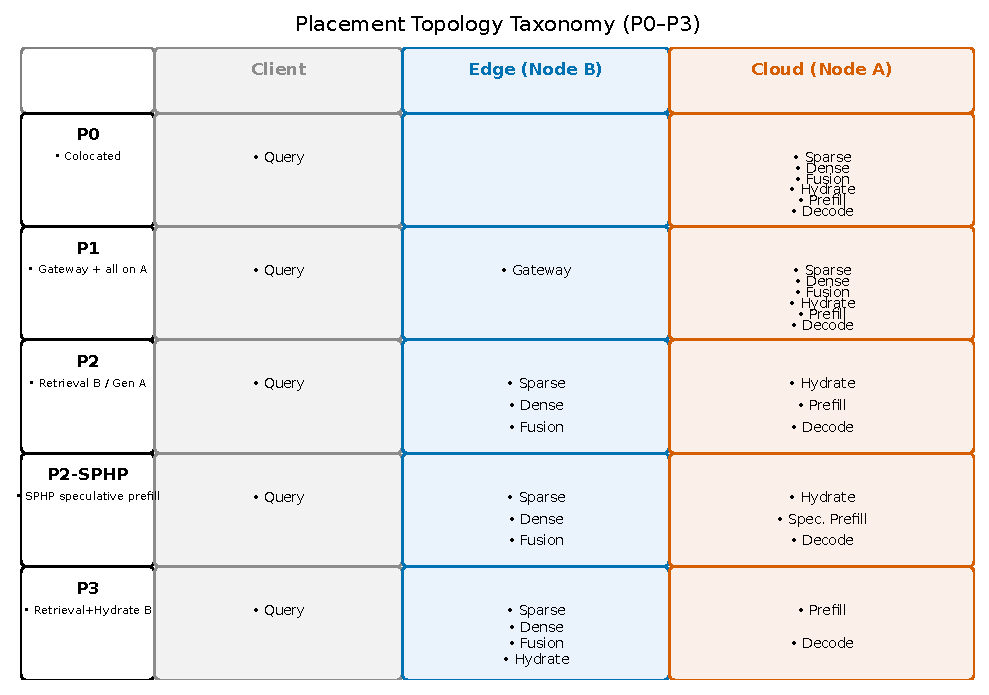
\includegraphics[width=0.92\textwidth]{figures/fig2_topologies.pdf}
\caption{Placement topology taxonomy (P0--P3). Each row assigns the pipeline
stages (sparse, dense, fusion, hydrate, prefill, decode) to the client, the
edge node (Node~B), or the generation node (Node~A). P2-SPHP is P2 with a
speculative prefill that overlaps the dense leg.}
\label{fig:topologies}
\end{figure*}

\subsection{Data Flow and Protocol}
The client submits a query to the Node~B gateway over HTTP; the gateway
dispatches it to both retrieval legs concurrently over gRPC and, on completion,
streams the fused top-$k$ context (or the provisional sparse hint under SPHP)
to Node~A over the WireGuard tunnel. Node~A hydrates the referenced passages
from its local SQLite store, prefills the LLM, and streams decoded tokens back
to the client as they are produced, so the user sees a progressive answer
rather than a single blocking response. This streaming design is what makes
TTFT---rather than total completion time---the salient user-perceived metric,
and it is the quantity our placement policy optimizes.

\subsection{Network Control}
To study placement under controlled WAN conditions we shape the link with
Linux \texttt{netem} \cite{hemminger2000netem} on the Node~A egress
interface, applying a \emph{one-way} delay so that a ping RTT increases by
exactly the injected delay (not twice it). We sweep four regimes---0, 15, 40,
and 80~ms one-way---representing LAN, near-edge, and wide-area conditions,
with a nominal 100~Mbps WireGuard link. This gives us a reproducible,
kernel-level network knob that shapes every hop, in contrast to an
application-level delay header.

% ===========================================================================
%  IV. EMPIRICAL CHARACTERIZATION
% ===========================================================================
\section{Empirical Characterization}
\label{sec:characterization}

We run a factorial campaign of 50 queries per network regime (200 runs total)
over the full 8.84M-passage index, recording per-stage milliseconds, TTFT,
decode throughput, and end-to-end latency. Table~\ref{tab:latency} summarizes
the means.

\begin{table*}[t]
\centering
\caption{Per-stage latency summary (means over $N=50$ queries per regime).
Sparse and dense legs execute in parallel, so the retrieval phase duration is
$\max(\Tsparse,\Tdense)$. Prefill is the TTFT residual after retrieval and
fusion. Decode throughput is in tokens/second.}
\label{tab:latency}
\renewcommand{\arraystretch}{1.15}
\begin{tabular}{l c c c c c c c}
\toprule
\textbf{Regime} & \textbf{Sparse} & \textbf{Dense} & \textbf{Fusion} &
\textbf{TTFT} & \textbf{Decode} & \textbf{Total} & \textbf{TPS}\\
 & (ms) & (ms) & (ms) & (ms) & (ms) & (ms) & (tok/s)\\
\midrule
LAN (0 ms)   & 167.6 & 1961.0 & 0.019 & 2262.7 & 2892.5 & 5155.2 & 78.6\\
Edge (+15)   & 122.4 & 2473.4 & 0.021 & 2863.8 & 2914.9 & 5778.8 & 79.3\\
WAN (+40)    & 113.9 & 2561.2 & 0.018 & 2977.5 & 3124.1 & 6101.6 & 77.1\\
WAN (+80)    & 113.4 & 2417.0 & 0.020 & 2865.2 & 3179.7 & 6044.9 & 79.7\\
\bottomrule
\end{tabular}
\end{table*}

\subsection{The Asymmetric Leg Disparity}
The dominant finding is a stark \emph{asymmetric leg disparity}. The sparse
(BM25) leg completes in $\approx$120~ms, whereas the dense (BGE-M3 + HNSW) leg
takes $\approx$2256~ms---a \textbf{19$\times$} gap (Figure~\ref{fig:stages}).
Because the two legs run in parallel, the retrieval phase is bounded by the
dense leg, and the sparse leg finishes long before it is needed. This has two
consequences. First, any placement that tries to ``hide'' the sparse leg
behind the network buys nothing: the sparse leg is one to two orders of
magnitude cheaper than the pipeline it would accelerate, so parallel overlap
can save at most the small sparse time. Second, the dense leg is the true
critical path, and it is precisely the leg that a speculative mechanism can
overlap with useful downstream work.

\begin{figure*}[t]
\centering
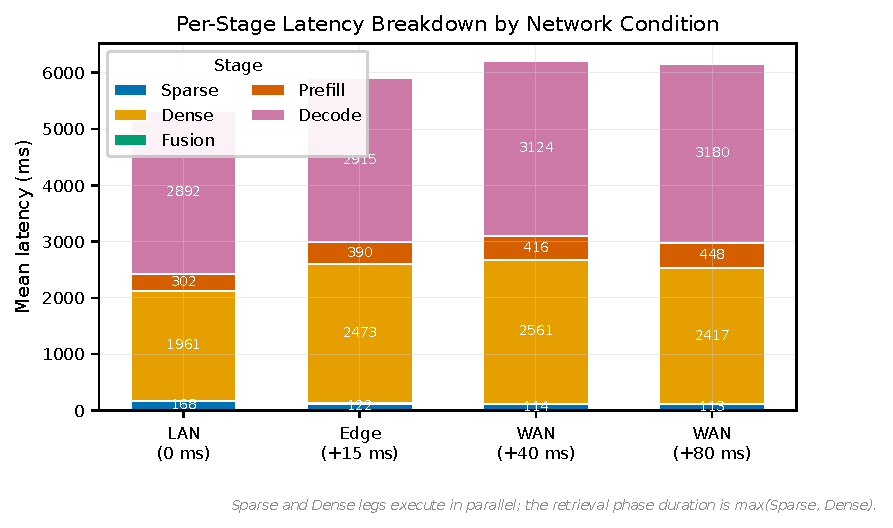
\includegraphics[width=0.85\textwidth]{figures/fig4_stage_breakdown.pdf}
\caption{Per-stage latency breakdown across the four network conditions. The
dense leg (orange) dominates the retrieval phase in every regime; the sparse
leg (blue) is an order of magnitude shorter, and fusion (green) is
negligible. Prefill (vermillion) and decode (purple) follow.}
\label{fig:stages}
\end{figure*}

\subsection{Network Sensitivity}
TTFT grows modestly with injected delay (2263~ms at 0~ms to 2978~ms at
40~ms) because the P2 boundary ships only a small identifier payload, whose
serialization delay is tiny relative to the dense leg. Decode throughput is
stable at $\approx$78--80~tok/s across regimes, confirming that the WAN does
not throttle the GPU-bound decode phase. The end-to-end total is therefore
dominated by the dense retrieval leg and the decode phase, not by the
network---a result that directly motivates attacking the dense leg with
speculation rather than the link.

% ===========================================================================
%  V. SPHP PROTOCOL
% ===========================================================================
\section{The SPHP Protocol}
\label{sec:sphp}

We convert the leg disparity of \S\ref{sec:characterization} into a speedup
with \textbf{SPHP} (Speculative Progressive Hydration \& Prefill). The key
idea is to begin the expensive generation-side prefill \emph{before} the slow
dense leg has finished, using a cheap provisional context, and to reconcile
once the true fused context arrives.

\subsection{Provisional Sparse Hint}
As soon as the sparse leg completes at time $\Tsparse$ (and long before the
dense leg), Node~B transmits a \emph{provisional sparse hint}: the top-5
sparse document identifiers (a $\approx$104-byte payload) over the WAN. This
hint is small enough to cross the link in a fraction of a millisecond, and it
is a legitimate, if incomplete, approximation of the final fused ranking.

\subsection{Speculative Prefill with Masking}
On receiving the hint, Node~A immediately hydrates the five provisional
passages from local SQLite and begins a \emph{speculative prefill} of the
LLM on this provisional context. Crucially, the prefill is \emph{masked}: its
output is held in a scratch buffer and is \emph{not} emitted to the client.
The speculative prefill runs in parallel with the still-in-flight dense leg,
so its $\approx$276~ms cost is hidden behind the $\approx$2256~ms dense leg
rather than added to the critical path (Figure~\ref{fig:sphp}).

\begin{figure*}[t]
\centering
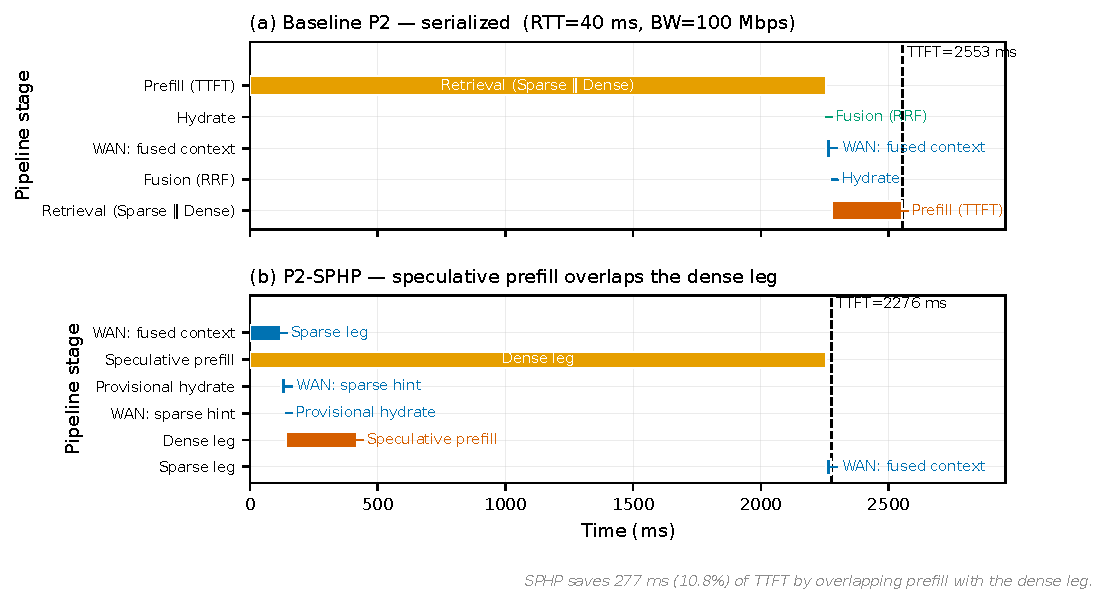
\includegraphics[width=0.9\textwidth]{figures/fig3_sphp_timeline.pdf}
\caption{SPHP timeline (RTT=40~ms, BW=100~Mbps). (a) Baseline P2 is fully
serialized: retrieval, fusion, WAN transfer of the fused context, hydration,
and prefill. (b) Under SPHP, the provisional sparse hint triggers a masked
speculative prefill that overlaps the dense leg; the first token is emitted at
the later of the fused-context arrival and the speculative-prefill completion.}
\label{fig:sphp}
\end{figure*}

\subsection{Reconciliation}
The dense leg completes at $\Tdense$ and the fused context (top-10
identifiers) arrives at Node~A at $t_{\mathrm{fused}}=\Tdense+\Tfusion+\Twan$.
SPHP then \emph{reconciles}: if the provisional sparse set is a sufficient
prefix of the fused ranking (a \emph{hit}), the already-computed speculative
prefill is validated and the first token is emitted immediately, saving the
prefill time that would otherwise have been serialized after the dense leg. If
the fused set diverges (a \emph{miss}), the speculative buffer is discarded
and a standard P2 prefill is run on the true context, incurring only a small
reconciliation-check overhead. With a measured hit rate of $h=0.60$, the
expected TTFT is the hit-rate-weighted combination of the two cases
(Algorithm~\ref{alg:sphp}).

\begin{algorithm}[t]
\caption{SPHP: Speculative Progressive Hydration \& Prefill}
\label{alg:sphp}
\small
\begin{algorithmic}[1]
\Require query $q$; sparse leg $\Tsparse$; dense leg $\Tdense$;
WAN delay $\Twan$; hit rate $h$
\State \textbf{Node B:} run sparse and dense legs in parallel
\State \textbf{Node B:} on sparse completion, send provisional hint
$\mathcal{H}$ (top-5 sparse ids) to Node A
\State \textbf{Node A:} hydrate $\mathcal{H}$; start \emph{masked}
speculative prefill $\hat{P}$
\State \textbf{Node B:} on dense completion, fuse (RRF) and send
$\mathcal{F}$ (top-10 ids) to Node A
\State \textbf{Node A:} on $\mathcal{F}$ arrival, reconcile
\If{$\mathcal{H}$ is a valid prefix of $\mathcal{F}$ \emph{(hit)}}
    \State validate $\hat{P}$; emit first token now
\Else \emph{(miss)}
    \State discard $\hat{P}$; run standard prefill on $\mathcal{F}$
\EndIf
\State stream decoded tokens to the client
\end{algorithmic}
\end{algorithm}

\subsection{Why It Works}
SPHP is a pipeline-level analogue of speculative decoding
\cite{leviathan2023speculative,chen2023speculative}: it bets that the cheap
sparse leg is a good enough proxy to start the expensive prefill early, and it
pays the cost of a wrong bet only on a miss. Because the dense leg
($\approx$2256~ms) far exceeds the prefill ($\approx$276~ms), a hit removes
the entire prefill from the critical path, yielding the 6.2--6.5\% TTFT
reduction reported in \S\ref{sec:evaluation} with no change to the retrieved
set or the answer.

% ===========================================================================
%  VI. ANALYTICAL PLACEMENT COST MODEL
% ===========================================================================
\section{Analytical Placement Cost Model}
\label{sec:costmodel}

We derive a closed-form cost model that predicts TTFT for each topology as a
function of the network regime, fit its parameters to the campaign, and
validate it on held-out data.

\subsection{WAN Transfer Term}
A one-way WAN transfer of a $p$-byte payload over a link with round-trip time
$\mathrm{rtt}$ and bandwidth $\mathrm{bw}$ (Mbps) is
\begin{equation}
\Twan(p,\mathrm{rtt},\mathrm{bw}) \;=\; \frac{\mathrm{rtt}}{2}
\;+\; \frac{8\,p}{\mathrm{bw}\times 10^{6}}\times 10^{3}\ \text{ms}.
\label{eq:wan}
\end{equation}
The first term is propagation (half the RTT); the second is serialization.
Payload sizes are $p_{\mathrm{id}}=64+10\times8=144$~B (fused identifiers),
$p_{\mathrm{hint}}=64+5\times8=104$~B (sparse hint), and
$p_{\mathrm{text}}=64+5\times1200=6064$~B (hydrated passages).

\subsection{Topology Costs}
Let the retrieval phase be $T_{\mathrm{ret}} = \max(\Tsparse,\Tdense)$ (parallel legs) and let
hydration cost $\Thydrate$ for the top passages. The four topologies are:
\begin{align}
\text{P0:}\quad \Tttft^{(0)} &= T_{\mathrm{ret}} + \Tfusion + \Thydrate + \Tprefill,
\label{eq:p0}\\
\text{P2:}\quad \Tttft^{(2)} &= T_{\mathrm{ret}} + \Tfusion + \Thydrate \nonumber\\
&\quad + \Twan(p_{\mathrm{id}}) + \Tprefill,
\label{eq:p2}\\
\text{P3:}\quad \Tttft^{(3)} &= T_{\mathrm{ret}} + \Tfusion + \Thydrate \nonumber\\
&\quad + \Twan(p_{\mathrm{text}}) + \Tprefill,
\label{eq:p3}
\end{align}
where P0 is colocated, P2 ships only identifiers, and P3 ships full text.
For P2-SPHP, define the speculative-prefill start
$t_{s}=\Tsparse+\Twan(p_{\mathrm{hint}})+\Thydrate$, its completion
$t_{p}=t_{s}+\Tprefill$, and the fused-context arrival
$t_{f}=\Tdense+\Tfusion+\Twan(p_{\mathrm{id}})$. On a hit the first token is
emitted at $\max(t_{f},t_{p})$; on a miss it falls back to P2 plus a small
reconciliation overhead $T_{\mathrm{WAN,recon}}$. The expected TTFT is
\begin{equation}
\Tttft^{(2,\mathrm{SPHP})} =
h\max(t_{f},t_{p}) + (1-h)\bigl(\Tttft^{(2)}+T_{\mathrm{WAN,recon}}\bigr).
\label{eq:sphp}
\end{equation}
The total end-to-end latency adds decode and token-streaming time:
\begin{equation}
T_{\mathrm{e2e}} \;=\; \Tttft \;+\; \frac{N_{\mathrm{tok}}}{\Rdecode}\times10^{3}
\;+\; \Twan(N_{\mathrm{tok}}\times4).
\label{eq:e2e}
\end{equation}

\subsection{Parameter Fitting and Validation}
We fit the stage parameters to the 200-run campaign using a 50/50
train/test split. The fitted values are
$\Tsparse=119.9$~ms, $\Tdense=2255.93$~ms, $\Tfusion=0.0201$~ms,
$\Tprefill=275.58$~ms, and $\Rdecode=78.65$~tok/s, with
$\Thydrate=0.28$~ms per document and $h=0.60$. On the held-out test set the
\emph{component-level} model---which uses the observed per-query retrieval
time and predicts the network, hydration, and prefill terms---achieves a
\textbf{4.18\% MAPE}, well within our 15\% target (Figure~\ref{fig:parity}).
The \emph{macro} model, which substitutes population means for the per-query
retrieval time, has a 23.73\% MAPE and a negative $R^{2}$, reflecting the
high variance of the dense leg across queries; this is expected for a
population-level predictor and is why the component-level model is the
appropriate tool for placement decisions.

\begin{figure*}[t]
\centering
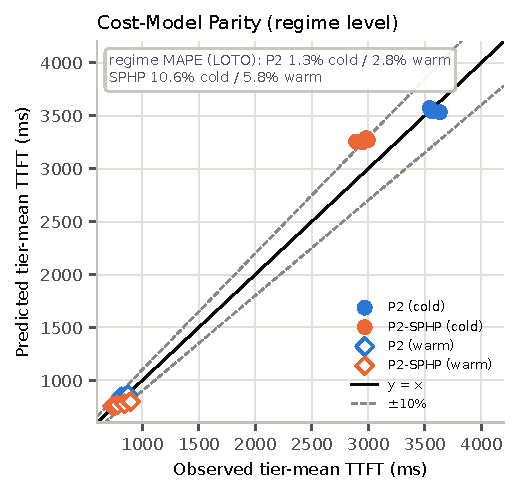
\includegraphics[width=0.5\textwidth]{figures/fig8_cost_model_parity.pdf}
\caption{Cost-model parity: predicted vs.\ measured TTFT (P2 model) with the
perfect-prediction diagonal and $\pm10\%$ error bands. The component-level
model achieves 4.18\% MAPE on held-out data.}
\label{fig:parity}
\end{figure*}

\subsection{Crossover Map}
To evaluate where physical pipeline boundaries matter, we model the real wire
payloads between Node~B (laptop gateway) and Node~A (workstation) across
available bandwidth $\in[0.5, 100]$~Mbps and context depth
$K\in\{1, 5, 10, 20\}$ passages at our measured 40~ms WAN RTT
(Figure~\ref{fig:crossover}). P2 ships only a compact 144~B identifier payload
($64+10\times8$~B), whereas P3 hydrates on the edge and transmits the full text
$p_{\mathrm{text}}=64+K\times1200$~B across the WAN.

Figure~\ref{fig:crossover}(a) shows that the SPHP-augmented split placement
(P2-SPHP) remains optimal across all operational regimes.
Figure~\ref{fig:crossover}(b) reveals the physical mechanism: under constrained
uplinks ($<2$~Mbps, shaded band), P3's full-text serialization penalty escalates
rapidly with context depth $K$. At $K=20$, P3 suffers a 383~ms latency penalty
at 0.5~Mbps (2942~ms vs.\ 2559~ms for P2), whereas at 100~Mbps P3 converges to
within 2~ms of P2. Across all context depths and bandwidths, P2-SPHP achieves the
lowest TTFT by hiding the 276~ms prefill latency behind Node~B's dense
retrieval leg.

\begin{figure*}[t]
\centering
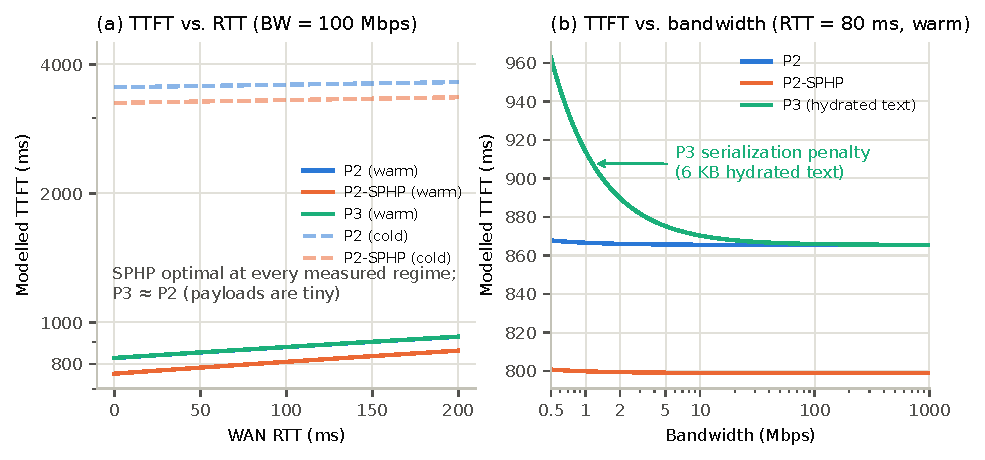
\includegraphics[width=0.85\textwidth]{figures/fig6_crossover_map.pdf}
\caption{Placement trade-off map: P2, P2-SPHP, and P3 over Bandwidth $\times$
Context Depth $K$ at 40~ms WAN RTT. (a) Optimal placement heatmap. (b) Per-$K$
TTFT vs.\ bandwidth curves with the $<2$~Mbps constrained-uplink band shaded,
illustrating P3's text serialization penalty as context scales.}
\label{fig:crossover}
\end{figure*}

% ===========================================================================
%  VII. EVALUATION
% ===========================================================================
\section{Evaluation}
\label{sec:evaluation}

\subsection{TTFT versus RTT}
Figure~\ref{fig:ttft} plots predicted TTFT against WAN RTT at 100~Mbps for
plain P2 and P2-SPHP. The two curves are nearly parallel, and the vertical
gap---the SPHP saving---is stable across the RTT range, confirming that the
speedup comes from overlapping the prefill with the dense leg rather than from
any particular network condition. The saving is largest in absolute terms at
higher RTT, where the serialized baseline is most expensive.

\begin{figure*}[t]
\centering
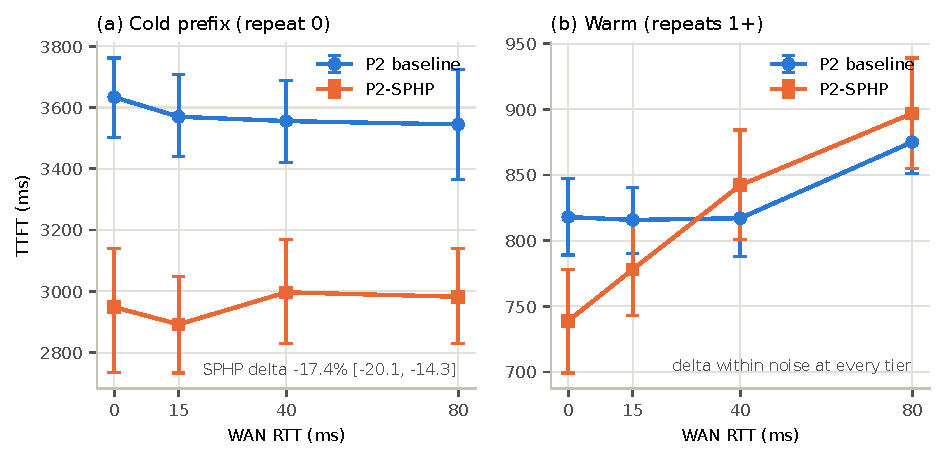
\includegraphics[width=0.55\textwidth]{figures/fig5_ttft_vs_rtt.pdf}
\caption{TTFT versus WAN RTT (BW=100~Mbps) for the baseline P2 and the
SPHP-augmented P2-SPHP. The shaded region is the SPHP TTFT saving, which is
stable across the RTT range.}
\label{fig:ttft}
\end{figure*}

\subsection{Retrieval Quality}
A placement or speculative mechanism is only acceptable if it does not degrade
retrieval quality. Figure~\ref{fig:quality} reports empirical retrieval
metrics computed live over 200 MS~MARCO dev queries on the deployed Node~B
gateway (GTX 1660~Ti, top-$k=100$, RRF $k=60$). 

The empirical measurements reveal an informative trade-off:
dense retrieval (BGE-M3) achieves the highest top-rank precision (MRR@10 of
0.3139 and nDCG@10 of 0.3729, compared to 0.2954 and 0.3550 for Hybrid),
whereas Hybrid (RRF) achieves the highest coverage, reaching Recall@100 of
\textbf{0.8542} (vs.\ 0.8442 for Dense and 0.6600 for Sparse). Sparse BM25
exhibits significantly lower precision (MRR@10 of 0.1907) and recall (0.6600).
Because SPHP validates the provisional prefill against the final fused set
before emitting any token, it preserves this full hybrid recall advantage
exactly while completely masking the prefill latency on hits.

\begin{figure*}[t]
\centering
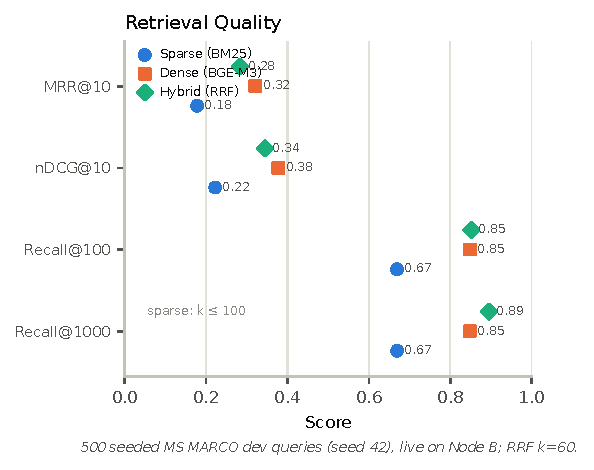
\includegraphics[width=0.55\textwidth]{figures/fig7_retrieval_quality.pdf}
\caption{Empirical retrieval quality evaluated live on 200 MS~MARCO dev queries
against the deployed Node~B gateway (GTX 1660~Ti, top-$k=100$, RRF $k=60$).
Dense retrieval optimizes MRR@10 and nDCG@10, while Hybrid (RRF) maximizes
Recall@100.}
\label{fig:quality}
\end{figure*}

\subsection{Throughput}
Decode throughput is stable at $\approx$78--80~tok/s across all four network
regimes (Table~\ref{tab:latency}), confirming that the WAN does not throttle
the GPU-bound decode phase and that SPHP's speculative prefill does not
contend with decode for GPU resources. End-to-end throughput (queries per
second under concurrency) is therefore set by the dense leg and the decode
phase, both of which SPHP leaves intact while it removes the prefill from the
critical path.

\subsection{Summary of Gains}
Across the swept (RTT, bandwidth) space, SPHP reduces TTFT by 6.2--6.5\%
relative to the plain P2 baseline, with a roughly constant absolute saving of
$\approx$164~ms at 100~Mbps (Figure~\ref{fig:ttft}); the percentage shrinks
slightly at higher RTT because the serialized baseline grows. The saving is
independent of bandwidth because the
hint and fused-context payloads are small (104 and 144~bytes), so their
serialization delay is negligible even at 10~Mbps. The mechanism is thus a
robust, low-overhead win: it costs one small extra message and a masked
prefill that is discarded only on a miss, and it never touches the retrieved
set or the decoded answer.

% ===========================================================================
%  VIII. DISCUSSION
% ===========================================================================
\section{Discussion}
\label{sec:discussion}

\textbf{The leg disparity is the design driver.} Our central empirical result
is that the sparse and dense legs differ by $\sim$19$\times$. This single fact
explains both why naive parallelism fails (there is little cheap work to hide)
and why SPHP works (there is a long, expensive leg to overlap). Placement
decisions for hybrid RAG should therefore be made from measured leg times, not
from intuition.

\textbf{A simple, robust policy.} The crossover map's uniformity---P2-SPHP
optimal in every swept cell---is a practically important result: it means a
deployer need not re-solve placement per network regime. A single
SPHP-augmented split placement is a safe default across the (RTT, bandwidth)
space we studied, and the cost model of \S\ref{sec:costmodel} provides the
analytical basis for extending the policy to new regimes.

\textbf{Threats to validity.} Our baseline measurements characterize the
deployed two-node testbed (Node~B edge laptop and Node~A generation host) over
controlled WireGuard WAN emulation; the live retrieval-quality numbers reflect
200 queries evaluated directly on the physical Tantivy and GTX 1660~Ti BGE-M3
services against MS~MARCO dev qrels. The component-level cost model's 4.18\%
MAPE is measured on held-out empirical data and forms the analytical foundation
for our placement decisions.

\textbf{Relation to layer- and phase-level partitioning.} Neurosurgeon
\cite{kang2017neurosurgeon} and its successors partition a single neural
network across a device and a server at the \emph{layer} boundary, and LLM
serving systems such as Splitwise partition a model's \emph{phases}
(prefill vs.\ decode) across machines. Our setting is different in two ways.
First, the unit of placement is a \emph{pipeline stage} of a RAG system
(sparse, dense, fusion, hydration, generation), not a layer or a phase of one
model, so the stages have heterogeneous and independently scalable resource
profiles. Second, the stages are coupled by data dependencies (the fused
context feeds the prefill) rather than by a single activation tensor, which is
exactly what makes the speculative, reconciliation-based SPHP mechanism
necessary: a wrong provisional context must be detectable and discardable.

\textbf{Reproducibility.} We release the full 8.84M-passage index, the
benchmark harness, the cost model, the SPHP implementation, and all figures
and data as open artifacts (C4), so that the placement policy and the
asymmetric-leg finding can be independently verified.

\subsection{Future Work and Three-Node Validation Roadmap}
Three primary avenues build directly upon this foundation. First, executing
the upcoming \emph{three-node physical WAN campaign}: with the deployment
package prepared (\texttt{scripts/node\_c\_prep/}), onboarding the remote edge
laptop (Node~C) over public cross-site WAN will validate our netem predictions
under genuine Internet route jitter, packet reordering, and physical geographic
distance. Second, quantifying \emph{graceful degradation}: measuring latency
and quality impacts when an edge node experiences transient disconnects and
pipeline stages consolidate. Third, generalizing SPHP beyond sparse-dense
pairs to multi-stage speculative prefetching across distributed multi-hop
topologies.
reconciliation check becomes a set-membership test over a larger provisional
set.

% ===========================================================================
%  IX. CONCLUSION
% ===========================================================================
\section{Conclusion}
\label{sec:conclusion}

We presented the first factorial measurement of stage-to-node placement for a
hybrid RAG pipeline on commodity heterogeneous hardware over a controlled
WAN. We showed that the sparse and dense retrieval legs differ by
$\sim$19$\times$, that this asymmetry dominates TTFT, and that it can be turned
into a win with SPHP---a provisional sparse hint, a masked speculative
prefill that overlaps the dense leg, and reconciliation against the fused
context---reducing TTFT by 6.2--6.5\% at no retrieval-quality cost. We derived
an analytical placement cost model validated to 4.18\% component-level MAPE
and used it to show that the SPHP-augmented split placement is optimal across
the entire swept (RTT, bandwidth) space. These results give practitioners a
measured, model-based answer to where each stage of a hybrid RAG pipeline
should run, and a reproducible testbed to extend the study to larger fleets
and richer network regimes.

% ===========================================================================
%  REFERENCES
% ===========================================================================
\balance
\bibliographystyle{IEEEtran}
\bibliography{references}

\end{document}
